%        File: TDDD14-lecture-notex.tex
%     Created: Mon Apr 04 10:00  2016 C
% Last Change: Mon Apr 04 10:00  2016 C
%
\documentclass[a4paper]{article}
\usepackage[utf8]{inputenc}
\usepackage{float}
\usepackage{graphicx}
\usepackage{hyperref}
\usepackage{amssymb}
\usepackage{mathtools}
\newtheorem{definition}{Definition}
\newtheorem{lemma}{Lemma}
\newtheorem{example}{Example}
\title{Lecture Notes\\TDDD14}
\author{Pontus Persson}
\date{VT-16}

\begin{document}
\maketitle
\tableofcontents
\marginpar{Lecture 1\\2016-04-04}
\section{Introduction}
Course questions:
\begin{itemize}
    \item What is a computer?
    \item What is their computational power?
    \item Programming languages
    \item Compilers
\end{itemize}
Some answers:
\begin{itemize}
    \item Different computational models leads to different computational powers
    \item Yes, there are problems which a computer can not solve
\end{itemize}
\subsection{Automata}
\textbf{Course backbone:} Automata\\
We use them to define formal languages and more importantly, computational models.
\\Many applications:
\begin{itemize}
    \item Artificial intelligence
    \item Vending machines
    \item Traffic lights, turnstile
    \item Video games
\end{itemize}
\begin{figure}[H]
    \centering
    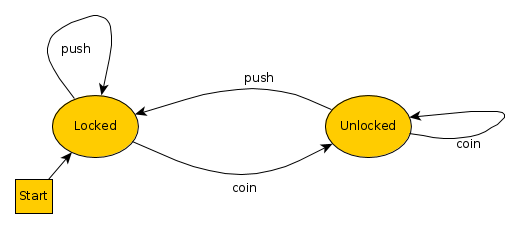
\includegraphics[width=0.9\textwidth]{turnstile.png}
    \caption{Turnstile Automata}
    \label{fig:turnstile}
\end{figure}
We treat mainly three types of automata:
\begin{enumerate}
    \item Finite memory (finite automata, FAs, e.g. turnstile)
    \item Infinite memory with restricted access (push-down automata, PDAs)
    \item Infinite memory without restricted access.
\end{enumerate}
\subsection{Some terminology}
Should be familiar with:
\begin{itemize}
    \item Sets and operations with sets
    \item Functions
    \item Relations
    \item Cartesian product
    \item Some sense of order and partial orders
    \item Equivalence relation
    \item Graphs and trees
    \item Binary and decimal repr. of numbers
\end{itemize}
\section{Basic definitions}
\begin{definition}
    A \textbf{decision problem} is a function with a one bit output: ``yes'' or ``no''.\\
    To specify a decision problem, we need two things:
    \begin{itemize}
        \item The set A of possible inputs
        \item The subset $B\subseteq A$ of ``yes'' instances
    \end{itemize}
\end{definition}
\begin{example}
    Given n, is n odd? Is a decision problem\\
    $A=\mathbb{N}$, $B=\left\{ n\in\mathbb{N} \middle| n\equiv 1 (mod 2) \right\}$\\
\end{example}
\begin{example}
    Given a,b. What is the greatest common divisor? Is not a decision problem.
\end{example}
In this course: an input is always a string of some alphabet.
\begin{definition}
    An \textbf{alphabet} is any finite set.\\
    We call the elements of this set symbols or letters. An alphabet is typically
    denoted with $\Sigma, \Gamma$. Symbols are often denoted with $a,b,c,\ldots$
\end{definition}
\begin{definition}
    A \textbf{string} over $\Sigma$ is any finite-length sequence of elements of $\Sigma$.\\
    We usually denote strings x,y,z,w,u,v,\ldots
\end{definition}
\begin{example}
    If $\Sigma=\left\{ a,b \right\}$, then ``aabab'' is a string over $\Sigma$ of length 5.
\end{example}

\begin{definition}
    The \textbf{length} of a string x is the number of symbols in x.\\
    Denoted by $|x|$.
\end{definition}
\begin{definition}
    The \textbf{null string} of \textbf{empty string} is denoted by $\epsilon$.\\
    $|\epsilon|=0$
\end{definition}
\begin{definition}
    Some terminology.
    \begin{itemize}
        \item $a^n$ A string of a's of length n ($a^5=aaaaa$, $a^0=^{def}\epsilon$)
        \item The set of all string over $\Sigma$ is denoted by $\Sigma^*$.
        \item $\emptyset^*=\left\{ \epsilon \right\}$
        \item If $\Sigma$ is non-empty then, $\Sigma^*$ is an infinite set of
            finite-length strings.
        \item Note: $\emptyset,\left\{ \epsilon \right\}, \epsilon$ are three
            \textbf{different} things.
    \end{itemize}
\end{definition}
\begin{definition}
    \textbf{Concatenation} takes two strings and x,y and creates a new string xy
            by putting them together end to end. xy is called the concatenation of x and y.\\
            \textbf{Note:} $xy \neq yx$ in general.
            \begin{itemize}
                \item Concatenation is associative: $(xy)z=x(yz)$
                \item $\epsilon$ is an identity for concatenation $\epsilon x=x\epsilon = x$
                \item $|xy|=|x|+|y|$
                \item $a^ma^n=a^{m+n}$
            \end{itemize}
\end{definition}
\begin{definition}
    We write $x^n$ for the string obtained by concatenating n copies of x.
\end{definition}
\begin{definition}
    If $a\in\Sigma$ and $x\in\Sigma^*$ we write $\#a(x)$ for the number
            of a's in x
\end{definition}
\begin{definition}
    A \textbf{prefix} of a string x is an initial substring of x.
\end{definition}
\begin{definition}
    A \textbf{suffix} of a string x is an ending substring of x.
\end{definition}
\begin{definition}
    The \textbf{complement} in $\Sigma^*$, $A\subseteq\Sigma^*$ is denoted by
    $~A=\left\{ x\in\Sigma^* \middle| x\notin A \right\}$, we denote it by $\hat{A}$.
\end{definition}
\begin{definition}
    Set concatenation $A,B\in\Sigma^*$, $AB=\left\{ xy \middle | x\in A, y\in B \right\}$
\end{definition}
\end{document}

